\clearpage

\section {Choice of oscillation parameters}
\label{sec:oscparamchoice}

This analysis departs from choices which have been followed historically in the T2K stand-alone $\nu_{e}$-appearance and 
$\nu_{\mu}$-disappearance analyses by changing the oscillation mixing parameters and the mass-squared splitting parameters.
There is a strong motivation for this change in the context of a joint 3-flavour analysis, and it is outlined below.

\subsection* {Neutrino mixing parameters}

In the stand-alone $\nu_{\mu}$-disappearance analysis, $\sin^{2}2\theta_{23}$ is typically measured since it appears in the 
first-order approximate formula for the $\nu_{\mu}$ survival probability:
\begin{equation}
P(\nu_{\mu}\rightarrow\nu_{\mu}) \approx 1 - sin^{2}2\theta_{23} sin^{2} \left(  \frac{\Delta m_{32}^{2} L}{4E_{\nu}}\right)
\end{equation}
In the stand-alone analysis, it is nearly impossible to distinguish $\theta_{23}$ from $\pi/2 - \theta_{23}$, 
as both inputs give the same value for $\sin^{2}2\theta_{23}$ and, therefore, the same $\nu_{\mu}$-survival probability 
This is the so-called octant ambiguity.

\begin{figure}[htbp]
\begin{center}
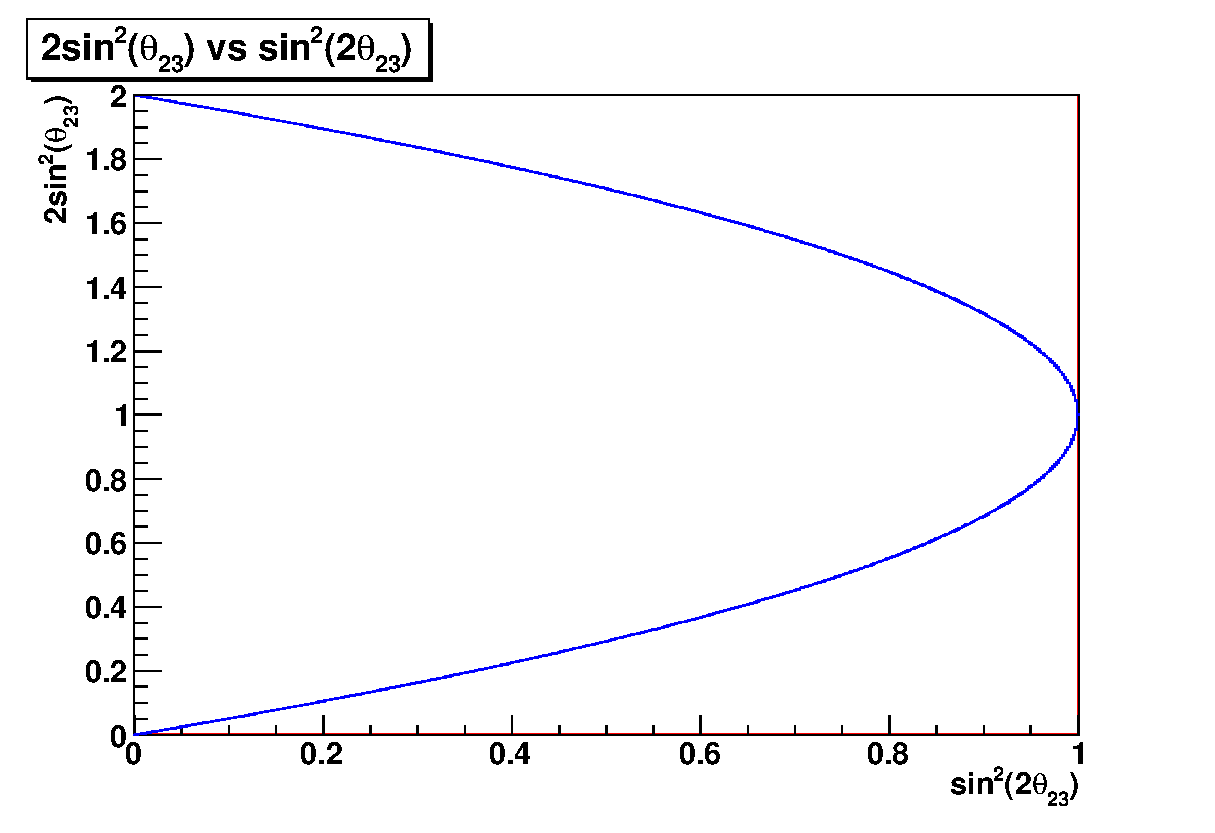
\includegraphics[width=0.5\textwidth]{images/description/Sin2thetaVsSin22theta.eps}
\caption{$\sin^{2}\theta_{23}$ (appears in leading-order term of P($\nu_{\mu}\rightarrow\nu_{e}$) vs $\sin^{2}2\theta_{23}$(
appears in leading-order term of P($\nu_{\mu}\rightarrow\nu_{\mu}$).}
\label{fig:ambig}
\end{center}
\end{figure}
Looking at the leading-order approximation of $P(\nu_{\mu}\rightarrow\nu_{e})$, the 23-sector mixing parameter appears as $\sin^{2}\theta_{23}$:
\begin{equation}
P(\nu_{\mu}\rightarrow\nu_{e}) \approx sin^{2}2\theta_{13}sin^{2}\theta_{23} sin^{2} \left(  \frac{\Delta m_{31}^{2} L}{4E_{\nu}}\right)
\end{equation}

\noindent
it is possible to lift the octant degeneracy by combining the $\nu_{\mu}$-disappearance and $\nu_{e}$-appearance analyses, as shown 
graphically in Fig.\ \ref{fig:ambig}. It is therefore a more natural choice for the joint 3-flavour oscillation analysis to fit for 
$\sin^{2}\theta_{ij}$ rather than $\sin^{2}2\theta_{ij}$, and this is the choice that has been implemented in the VALOR analysis framework.
The option to fit for $\sin^{2}2\theta_{ij}$ has also been retained for backward compatibility and to allow validation checks.

%
%variables in global fits performed by theorists \cite{LisiGlobalAnalysis}, \cite{ConchaMaltoniGlobalAnalysis}, 
%and was already suggested in the collaboration by Mauro Mezzetto and others. 
%Some experiments in the past already used variables in $sin^{2}\theta$ (or $tan^{2}\theta$) 
%such as KamLAND \cite{KamLAND2008Paper}. 
%This choice of the mixing angles will make possible the study of the octant degeneracy of the 
%parameter $\theta_{23}$ as it has been introduced in this note and discussed in 
%several presentations for analysis meetings; however the analysis for the octant 
%degeneracy is going to be described in the documentation for next 2012 joint oscillation analysis. 
%

% Mass square splitting parameters
\subsection* {Mass-squared splitting parameters}
\label{sec:masschoice}

Previous T2K analyses have used the following mass-squared splitting parameters:
\begin{center}
$\left( |\Delta m_{32}^{2}|, \Delta m_{21}^{2} \right)$ 
\end{center}
which are defined as $\Delta m_{ij}^{2} = m_{i}^{2} - m_{j}^{2}$ according to the PDG notation \cite{PDG}. 
The mass hierarchy is set through the sign of $\Delta m_{32}^{2}$
i.e.\ $\Delta m_{32}^{2} = |\Delta m_{32}^{2}|$ in the normal hierarchy 
and $\Delta m_{32}^{2} = - |\Delta m_{32}^{2}|$ in the inverted hierarchy. 
The remaining mass-squared splitting is defined as $\Delta m_{31}^{2} = \Delta m_{32}^{2} + \Delta m_{21}^{2}$ for both hierarchies.

In the normal hierarchy (NH) $m_{1}^{2}<m_{2}^{2}<<m_{3}^{2}$, while in the inverted hierarchy (IH) $m_{3}^{2}<<m_{1}^{2}<m_{2}^{2}$,
i.e.\ $|\Delta m_{31}^{2}|$ is the largest mass-squared splitting in the NH, whereas $|\Delta m_{32}^{2}|$ is the largest in the IH. 
This means that it is not possible to compare the two hierarchies if the atmospheric mass-squared difference is input as 
$|\Delta m_{32}^{2}|$. This has been pointed out by several authors and different schemes are typically employed in global
oscillation fits to circumvent this issue. The VaLOR joint oscillation analysis uses the scheme defined by Fogli and Lisi in 
\cite{LisiGlobalAnalysis} \cite{Fogli} in which $\left( |\Delta m_{32}^{2}|, \Delta m_{21}^{2} \right)$ are replaced by:
\begin{center}
$\left( |\Delta m^{2}|, \delta m^{2} \right)$
\end{center}
where 
$\Delta m^{2} = \left(m_{3}^{2} - \frac {m_{1}^{2}+m_{2}^{2}} {2} \right) =  \left( \frac {\Delta m_{31}^{2} + \Delta m_{32}^{2}} {2} \right)$
and 
$\delta m^{2} = \Delta m_{21}^{2}$.
$|\Delta m^{2}|$ is the "atmospheric" squared-mass splitting, which has the same absolute value for both mass hierarchies.
$\delta m^{2}$ is the "solar" squared-mass splitting which is known to be positive. When the mass-squared splittings are input as 
$\left(\Delta m^{2}, \delta m^{2} \right)$, the mass hierarchy is set through the sign of $|\Delta m^{2}|$, and $\Delta m_{32}^{2}$ 
and $\Delta m_{31}^{2}$ are calculated as 
\begin{displaymath}
\begin{split}
\Delta m_{32}^{2} &= \Delta m^{2} - \frac{\delta m^{2}}{2}  \\
\Delta m_{31}^{2} &= \Delta m^{2} + \frac{\delta m^{2}}{2}
\end{split}
\end{displaymath}
for both mass hierarchies. The ability to input the mass-squared differences as $\left( |\Delta m_{32}^{2}|, \Delta m_{21}^{2} \right)$ has also been retained for 
backward compatibility and to allow various validation checks.

The effects of changing the convention for the inputs of the mass-squared splitting parameters on P($\nu_{\mu}\rightarrow\nu_{\mu}$) 
and P($\nu_{\mu}\rightarrow\nu_{e}$) are shown in Fig.\ \ref{fig:oscprobmassdef}. 

\begin{figure}[htbp]
\begin{center}
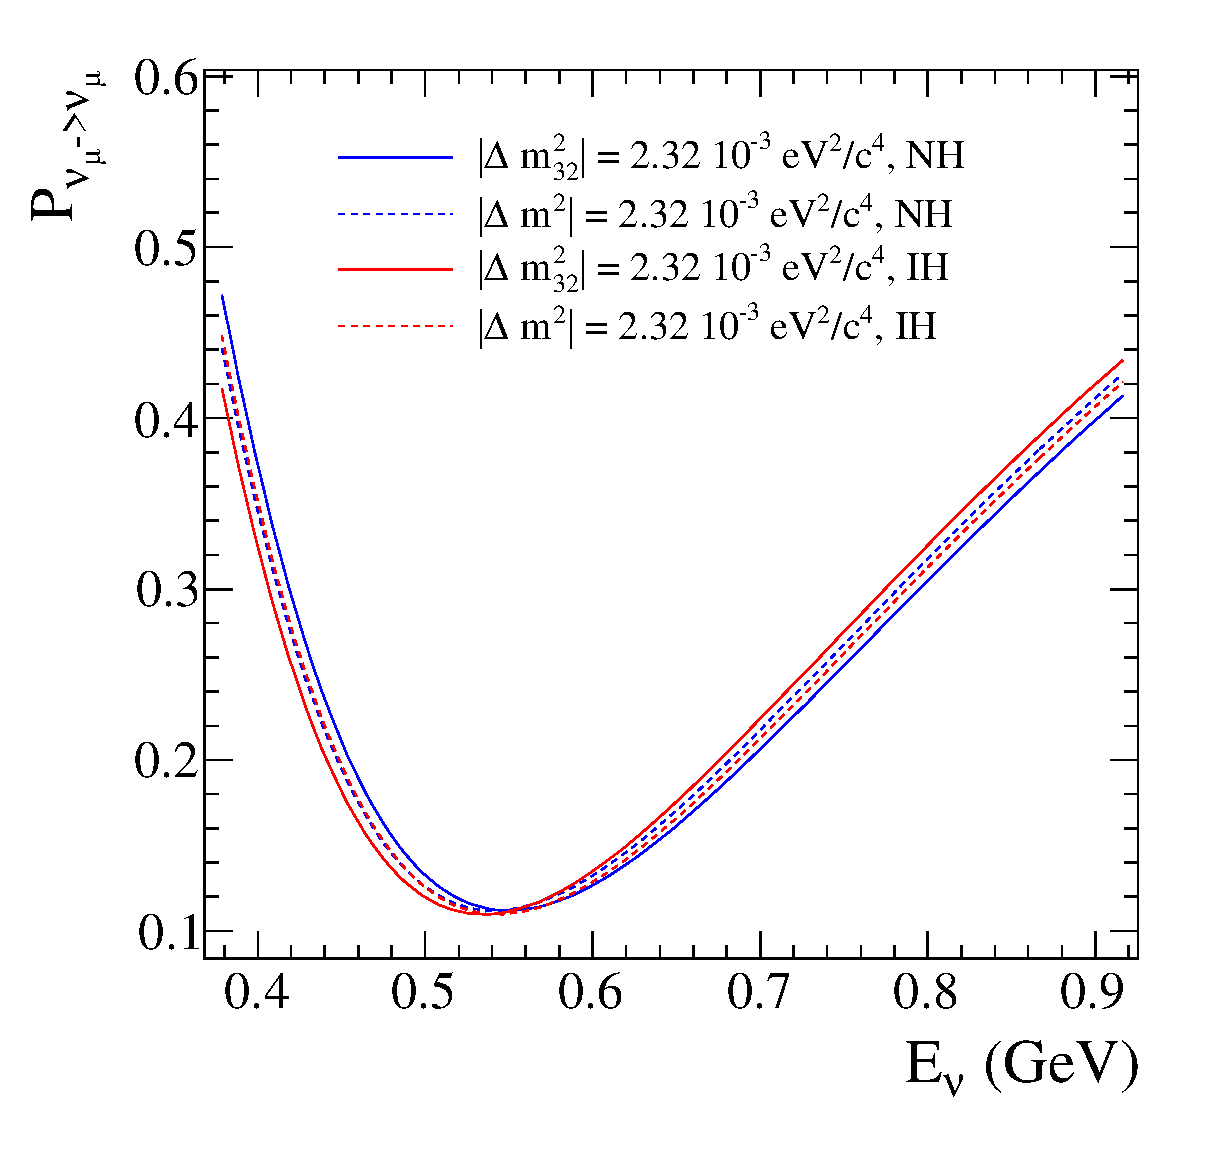
\includegraphics[width=0.5\textwidth]{images/description/OscProbNuMuNuMuMassDef.eps}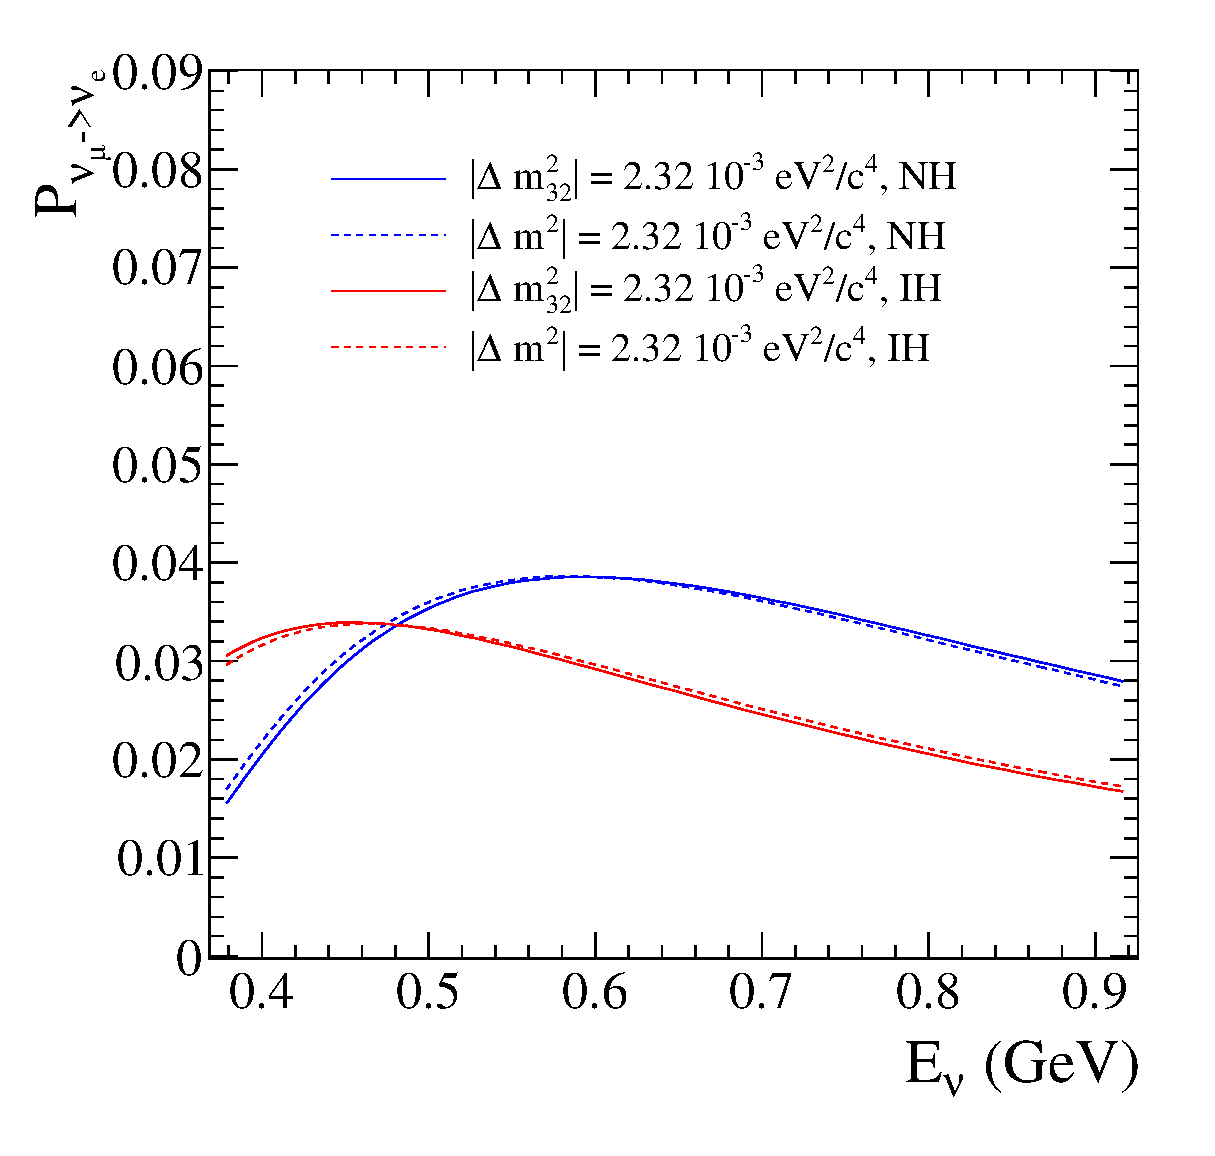
\includegraphics[width=0.5\textwidth]{images/description/OscProbNuMuNuEMassDef.eps}
\caption{
Effects of changing the convention for the inputs of the mass-squared splitting parameters on P($\nu_{\mu}\rightarrow\nu_{\mu}$) (left) and 
P($\nu_{\mu}\rightarrow\nu_{e}$) (right): $|\Delta m_{32}^{2}|$ = 2.32$\times$10$^{-3}$ eV$^{2}$/c$^{4}$ (solid lines) and $|\Delta m^{2}|$ 
= 2.32$\times$10$^{-3}$ eV$^{2}$/c$^{4}$ (dashed lines) for the normal hierarchy (blue) and inverted hierarchy (red). 
 The other oscillation parameters are $\sin^{2}2\theta_{12}$ = 0.857, $\delta m^{2}$ = 7.5$\times$10$^{-5}$ eV$^{2}$/c$^{4}$, 
 $\sin^{2}2\theta_{13}$ = 0.098 (2012 PDG values), $\delta_{CP}$ = 0 and $\sin^{2}2\theta_{23}$ = 0.9. 
}
\label{fig:oscprobmassdef}
\end{center}
\end{figure}

Section \ref{app:fogliandlisi} illustrates the difference in the comparison between results in the two mass hierarchies when using
the Fogli and Lisi convention $\left( |\Delta m^{2}|, \delta m^{2} \right)$ and the previous convention $\left( |\Delta m_{32}^{2}|, \Delta m_{21}^{2} \right)$. 


%Table \ref{tab:numeventsmassdef} shows the predicted number of events of the $1R_{e}$-like events and $1R_{\mu}$-like events using the values from 
%PDG2012 for the oscillation parameters, $sin^{2}2\theta_{12}=0.857, \delta m^{2}=7.50 \times 10^{-5} eV^{2}/c^{4}, sin^{2}2\theta_{13} = 0.098, \delta_{CP}=0$, 
%with $sin^{2}2\theta_{23} =0.9$, changing the mass hierarchy and the mass-squared convention 
%so that either $|\Delta m_{32}^{2}| =2.32 \times 10^{-5} eV^{2}/c^{4}$ or $|\Delta m^{2}| =2.32 \times 10^{-5} eV^{2}/c^{4}$. 
%
%\begin{table}[htbp]
%\begin{tabular} {|p{1cm}|p{1.7cm}|p{1.7cm}|p{1.7cm}|p{1.7cm}||p{1.7cm}|p{1.7cm}|p{1.7cm}|p{1.7cm}|}
%\hline
%  & \multicolumn{4}{|c||} {$1R_{e}$-like events }& \multicolumn{4}{|c|}{ $1R_{\mu}$-like events} \\
% \hline \hline
% &  $|\Delta m_{32}^{2}|$  NH & $|\Delta m^{2}|$ NH & $|\Delta m_{32}^{2}| $ IH & $|\Delta m^{2}| $ IH &  $|\Delta m_{32}^{2}|$ NH & $|\Delta m^{2}|$ NH & $|\Delta m_{32}^{2}|$ IH & $|\Delta m^{2}| $ IH \\
%\hline \hline
%Total  & 10.984 & 10.985 & 9.437 & 9.489 & 60.940 & 61.842 & 62.656 & 61.652 \\
%\hline 
%$\nu_{\mu}$  &  1.213 &  1.214 & 1.216 & 1.214 & 56.860 & 57.730 & 58.530 & 57.560 \\
%\hline
%$\bar{\nu_{\mu}}$  & 0.067 & 0.067 & 0.067 &  0.067 & 3.812 & 3.851 & 3.885 & 3.845 \\
%\hline
%$\nu_{e}$  & 1.509 & 1.510 & 1.526 & 1.525 & 0.135 & 0.135 & 0.135 & 0.135 \\
%\hline
%$\bar{\nu_{e}}$  &  0.079 & 0.079 &  0.079 & 0.078 & 0.013 & 0.013 &  0.013 & 0.013 \\
%\hline
%osc. $\nu_{e}$ & 8.117 & 8.116 & 6.551 & 6.604 & 0.118 &  0.118 & 0.096 & 0.097 \\
%\hline
%\end{tabular}
%\caption{Table of predicted number of events of the $1R_{e}$-like events and $1R_{\mu}$-like events using the values from PDG2012 for the oscillation parameters, $sin^{2}2\theta_{12}=0.857, \delta m^{2}=7.50 \times 10^{-5} eV^{2}/c^{4}, sin^{2}2\theta_{13} = 0.098, \delta_{CP}=0$ , with $sin^{2}2\theta_{23} =0.9$, changing the mass hierarchy and the mass-squared convention so that either $|\Delta m_{32}^{2}| =2.32 \times 10^{-5} eV^{2}/c^{4}$ or $|\Delta m^{2}| =2.32 \times 10^{-5} eV^{2}/c^{4}$}
%\label{tab:numeventsmassdef}
%\end{table}
%


\subsection* {Treatment of solar (12-sector) oscillation parameters}

A study has been made in which $\sin^{2}2\theta_{12}$ and $\Delta m_{21}^{2}$ were allowed to float in the fit of the single $\mu$-like ring Super K sample, and 
the results are shown in Appendix \ref{app:solar}. It was found that the fitter returned extreme values of these parameters (see Fig.\ \ref{fig:solarfit}), and 
this is because they have no effect on the single $\mu$-like ring sample. For this reason, these parameters were fixed throughout this analysis to the values 
in table \ref{tab:solarparameters}.

\begin{table}[h]
\centering
\begin{tabular}{|c|c|}
\hline
Parameter & Value \\
\hline
\hline
$\sin^{2}2\theta_{12}$ & 0.857 \\
\hline 
$\sin^{2}\theta_{12}$ & 0.311 \\
\hline 
$\Delta m_{21}^{2}$ & 7.5$\times$10$^{-5}$ eV$^{2}$/c$^{4}$ \\
\hline
\end{tabular}
\caption{Values used for $\sin^{2}2\theta_{12}$ and $\Delta m_{21}^{2}$ in the joint oscillation analysis}
\label{tab:solarparameters}
\end{table}



